%%% template.tex
%%%
%%% This LaTeX source document can be used as the basis for your technical
%%% paper or abstract. Intentionally stripped of annotation, the parameters
%%% and commands should be adjusted for your particular paper - title,
%%% author, article DOI, etc.
%%% The accompanying ``template.annotated.tex'' provides copious annotation
%%% for the commands and parameters found in the source document. (The code
%%% is identical in ``template.tex'' and ``template.annotated.tex.'')

\documentclass[]{acmsiggraph}
\usepackage{algorithm}
\usepackage[noend]{algpseudocode}
\TOGonlineid{45678}
\TOGvolume{0}
\TOGnumber{0}
\TOGarticleDOI{0}
\TOGprojectURL{}
\TOGvideoURL{}
\TOGdataURL{}
\TOGcodeURL{}
\usepackage{color}
%\definecolor{red}{rgb}{0.9, 0.17, 0.31}
\usepackage{multirow}
\usepackage{subfig}
\usepackage{xcolor}
\usepackage{lipsum}
\usepackage{listings}
\usepackage{graphicx}
\usepackage{glsllst} % My own package providing markup listing for glsl
\usepackage{rmlst}   % My own package providing markup listing for renderman
\usepackage{amsmath}
\usepackage{hyperref}

\lstset{
	backgroundcolor=\color[rgb]{0.95, 0.95, 0.95},
	tabsize=3,
	%rulecolor=,
	basicstyle=\footnotesize\ttfamily,
	upquote=true,
	aboveskip={1.5\baselineskip},
	columns=fixed,
	showstringspaces=false,
	extendedchars=true,
	breaklines=true,
	prebreak = \raisebox{0ex}[0ex][0ex]{\ensuremath{\hookleftarrow}},
	frame=none,
	aboveskip=15pt,
	belowskip=8pt,
	captionpos=t,
	showtabs=false,
	showspaces=false,
	showstringspaces=false,
	identifierstyle=\ttfamily,
	%keywordstyle=\color{red}\bfseries,
	%keywordstyle=[1]\bfseries\color{syntaxBlue},
	%keywordstyle=[2]\bfseries\color{syntaxRed},
	%keywordstyle=[3]\color{blue}\bfseries,
	%keywordstyle=[4]\bfseries\color{syntaxBlue},
	commentstyle=\color[rgb]{0.082,0.639,0.082},
	keywordstyle=[1]\bfseries\color[rgb]{0,0,0.75},
	keywordstyle=[2]\bfseries\color[rgb]{0.5,0.0,0.0},
	keywordstyle=[3]\bfseries\color[rgb]{0.127,0.427,0.514},
	keywordstyle=[4]\bfseries\color[rgb]{0.4,0.4,0.4},
	stringstyle=\color[rgb]{0.639,0.082,0.082},
}

\title{Innovations Report: Procedural Fur System}

\author{Joe Withers\thanks{e-mail:joewithers96@gmail.com}\\National Centre for Computer Animation}
\pdfauthor{Joe Withers}

\keywords{rendering}

\begin{document}

\maketitle

\begin{abstract}
For this project I developed a procedural fur system, with the aim of exploring the feasibility of offloading computation onto the GPU within artist tools. The final artefact is an application which serves to interface with the fur system API which I have developed. This report primarily documents the implementation of the API, as well as my findings.
\end{abstract}

\section{Introduction} \label{sec:introduction}
Introduction Text.
\subsection{Related work} \label{sec:related}

nvidia hairworks

\subsection{Existing solutions} \label{sec:existing}
Whilst many larger companies opt to develop their own software for handling fur, such as MPC's Furtility~\cite{furtility}, there are a number of commercially available solutions that are also widely used in production.

The most popular of these is XGen~\cite{xgen}, originally developed by Walt Disney Animation Studios, which has been included in Autodesk's Maya since 2014. XGen uses a 'Collection' and 'Description' paradigm; Descriptions store user controlled parameters which affect fur primitives (curves for example) on a select area of a mesh, and Collections act as a container for these Descriptions. There are two primary methods offered for distributing primitives on a mesh, Guide Curves can be used to manually control the placement and shape of primitives by placing 'Guides' on the mesh surface, whereas 'Groomable Splines' randomly distirbutes splines over the mesh surface which can be manipulated in real time using viewport manipulators that mimic the brushing and styling of fur. In both modes, 'modifiers' can be added to the modifier stack to further adjust the visual outcome, adding features such as clumping, noise, and coiling. Attributes within these modifiers can be further controlled using expressions or texture maps.

Another commercially available solution is Yeti~\cite{yeti}, which is also offered as a plugin within Autodesk's Maya. Yeti offers a more procedural approach, giving the user a node graph interface in which to construct the desired look from individual components. For example, the most simple usage requires the user to first create a 'scatter' node to distribute points on the mesh surface, and then combine it with a 'grow' node to extrude curves from these points. Whilst at first this may seem unintuitive when compared to XGen, it offers greater flexibility and avoids the pitfalls associated with a destructive workflow.

Offerering even more flexibility, recent versions of SideFX's Houdini include hair and fur operator nodes, which create predefined node networks for the generation of hair and fur. These networks use standard Houdini nodes internally, so experienced Houdini users are intuitively able to create the visual outcome they desire, using tools they already know. However, it may be quite unintuitive for asset artists (those who would be using the tool, Groom artists?), who are not used to Houdini's heavily procedural workflow.

\subsection{GPU acceleration} \label{sec:existingGPU}
Whilst it is not clear to what extent each of these solutions make use of GPU acceleration, they all perform fast enough to allow the user to manipulate them interactively. I therefore decided to monitor the CPU and GPU usage using \verb|htop| and \verb|nvidia-smi| respectively, before and after adding XGen content to a simple maya scene, to determine where the majority of data was being computed.

After applying the default XGen description onto a simple sphere with 760 triangles, there was no noticeable increase in both GPU utilisation and GPU memory usage. Increasing the density of the primitives from 1.0 to 10000.0 saw an increase of VRAM usage of roughly 350MiB, which I would attribute to storing the primitives in a buffer on the GPU, but there was no discernable increase in GPU utilisation. Increasing the density further to 10,000 saw a noticable spike in CPU usage, hitting 100 percent across two threads, leading me to believe that the primitive distribution computation is being done on the CPU.

However, when applying modifiers to the XGen description I noticed a small increase of roughly 2MiB in VRAM usage for the first modifier, yet no further increases for modifiers added after that. As this increase is quite small I would attribute it to storing the modifier attributes on the GPU, though I still noticed spikes in CPU usage when recalculating the XGen description once the modifier was added, which makes it inconclusive as to whether XGen uses any kind of GPU acceleration.

% on maya load: CPU up to 8 percent when moving mouse GPU very low but 40 percent when moving viewport 42MiB
% before xgen on sphere 36mib
% xgen on sphere density 1.0 36mib GPU
% xgen on sphere density 100.0 40mib GPU
% xgen CPU spiked up to 100 on a single thread when changing density
% xgen on sphere density 1000.0 56mib GPU
% xgen noise on sphere density 1000.0 63mib GPU, CPU spiked but only to 20%
% xgen on sphere density to 10,000 caused spike on 2 threads

\section{Implementation} \label{sec:implementation}
From my research it was clear that there is an apparent lack of standalone software for authoring fur; it makes sense that existing fur software are developed as software plugins, allowing the tool to make use of their host DCCs existing functionality.

However, by developing the system as a simple API one could make it DCC agnostic, which is why I chose to develop my system as a pairing of a simple API with a standalone tool which interfaces with it. By developing a simple API it could allow for future implementations as plugins within DCCs, providing the data exchange formats are compatible with the host DCC.

\subsection{Resources} \label{sec:resources}
I decided to develop the API side of the fur system using C++, primarly as it most commonly used when developing computationally heavy artist tools, but also because it is the language I am most comfortable using. I opted to use OpenGL over other APIs (CUDA, OpenCL) for offloading of computation onto the GPU, simply because my final artefact is a tool with a graphical interface, and OpenGL is capable of handling both arbitary computation using compute shaders and rendering of geometry simultaneously.

To handle the user interface I used the Qt framework within C++. Qt is commonly used for artist tools within visual effects as it is cross-platform, and applications can be configured to run within other applications that make use of it, such as Autodesk Maya.

I wanted to include a node-graph style interface within my application, as it is commonly used within existing artist tools (Autodesk Maya, Unreal Engine), and would encourage modularity within my API. Qt does not natively provide this kind of interface, so I made use of NodeEditor~\cite{Pinaev2017}, an existing Qt-based library that provides this functionality.

\subsection{Design} \label{sec:design}
From looking at existing fur systems I was able determine that my simplified fur system would need to consist of the following components:

\begin{itemize}
	\item Geometry Loaders - These are responsible for loading user specified geometry. Example Geometry Loaders could allow for the parsing of Wavefront OBJ files.
	\item Distributors - These are responsible for the distribution of curves onto user specified geometry. User controllable parameters could include density (curve count), distribution pattern (random, uniform), and curve length. These parameters could potentially be controlled by texture inputs.
	\item Operators - These are responsible for manipulation of the curves to achieve the desired look. Example operators could provide bending, clumping, or randomisation of input curves. These should behave much like the 'Modifiers' in XGen.
	\item Renderers - These are responsible for the rendering of curves into the application viewport. Example renderers could provide mesh, cuves as lines, or curves as ribbons rendering functionality. User controllable parameters could provide controls for the shading model in use, as well as control of the base and tip widths when rendering curve ribbons for example.
\end{itemize}

Whilst the list of components specified above provide the required functionality for a standalone tool, they do not provide any functionality for exporting fur for use in a broader pipeline. I chose to omit this functionality to limit the scope of this assignment, but the ability to export hair curves as alembic would be desirable, as alembic is a widely adopted format that allows for the storage of multiple different types of curve geometry. Another candidate file type would be RenderMan's RIB format, which would allow for direct rendering of the hair curves in any RenderMan compliant renderer.

\subsection{Development} \label{sec:development}

In this section I will explain the development of each of the major components, not necessarily in chronological order, but in the order regarding to how their data is passed through the system.

% write about distributing https://stackoverflow.com/questions/9294316/
% distribute-points-on-mesh-according-to-density

% write about GPU

\subsubsection{Mesh loading} \label{sec:objLoading}
% The first problem I tackled was that of loading mesh geometry into the system, and storing it in a Shader Storage Buffer Object (SSBO) for later use in a compute shader. I opted to implement a Wavefront OBJ loader as they are (deceptively) simple to parse, consisting of a list of vertex positions, vertex normals, vertex texture coordinates, and faces defined as a list of indices. I created an OBJ loader node using the NodeEditor library, which parses

The first problem I tackled was that of loading mesh geometry into the system, in such a way that would allow for later computation on both the GPU and CPU. I opted to implement a Wavefront OBJ loader as they are (deceptively) simple to parse, consisting of a list of vertex positions, vertex normals, vertex texture coordinates, and faces as defined by a list of indices. This data structure formed the basis of my 'Mesh' class. Using the NodeEditor library I then created a node which loads OBJ files, and outputs the 'Mesh' object through it's output data port.

\subsubsection{Curve distributors} \label{sec:distributors}

In order to generate curves for the system to manipulate, it was necessary to create a node that handles the distribution of curves onto the surface of a mesh. This node needs to take 'Mesh' object data as input, and output 'Curves' object data. A 'Curves' object was implemented which consists an array of 'Curve' objects, which in turn consist of an array 5 vertex positions that construct the curve. Distributor nodes would also need to alternate between performing the distribution process on the CPU or on the GPU, which would in turn affect whether the node outputs a 'Curves' object, or an ID for where the curves data is stored on the GPU.

With these parameters in mind I decided to implement an abstract distributor node class, which contains a virtual function for performing the distribution, and handles the callbacks for when input data is changed and the distribution needs to be updated. This makes the system somewhat extensible, allowing for different distribution patterns to be implemented with ease. The node's data type was also extented to be able to store either 'Curves' objects from the CPU, or an ID for an OpenGL buffer object, with an enumerated value to identify which of these is currently in use. This not only allows the distributor to alternate between CPU and GPU computation arbitrarily, but also allows nodes recieving this data to process it accordingly.

There are many different methods one could use to distribute points on an abritrary mesh, however for replicating creature fur it is desirable to choose a method that distributes primitives at random positions across the surface, yet roughly evenly spaced from neighboring primitives. A popular method used to achieve this kind of distribution is referred to as 'Dart Throwing', which relies on checking the distance to neighboring samples after a new sample has been generated, and discarding the sample if the samples are too close. Whilst these kinds of methods produce good results, they can be inefficient as in certain situations many samples may be generated and rejected, before a sample is accepted. An optimisation for this is described in \textit{Dart Throwing on Surfaces}~\cite{dartThrowing}, which relies on removing areas of the mesh that are already covered by a sample, by means of triangle subdivision.

Unfortunately, parallelizing dart thowing methods is not trivial, making them unsuitable for my desired usage of OpenGL compute shaders. Whilst sampling methods suitable for parallel processing do exist, such as those described in \textit{Parallel Poisson Disk Sampling with Spectrum Analysis on Surfaces}~\cite{parallelPoisson}, I instead opted to implement a naive random sampling method as it was much easier to parallelize.

\begin{figure}[htbp]
\centering
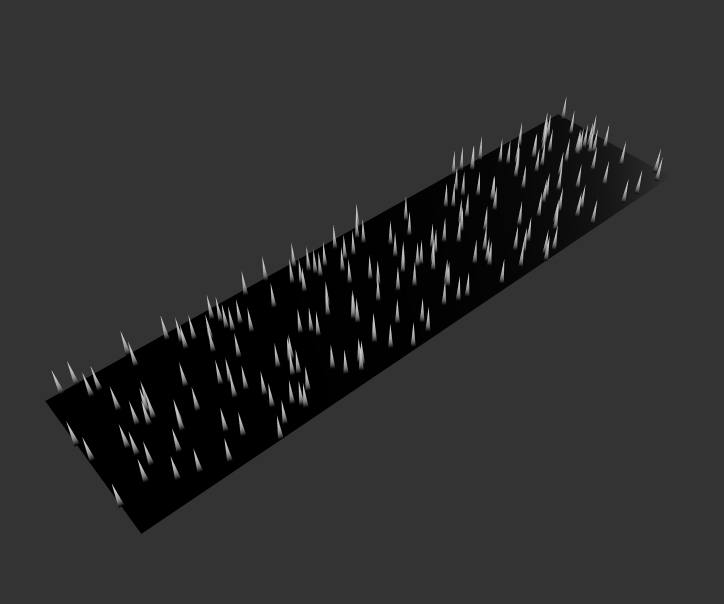
\includegraphics[width=0.49\linewidth]{images/triangleStripDistribution}
\hfill
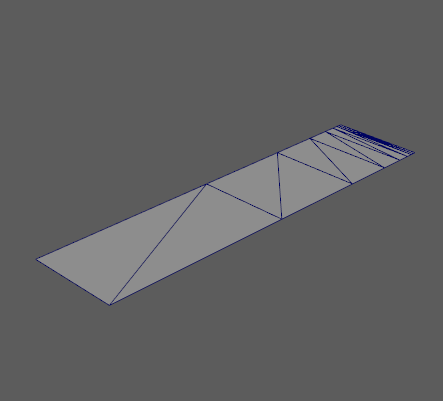
\includegraphics[width=0.45\linewidth]{images/triangleMesh}
\caption{\label{figure:distribution} Example distribution generated by my naive random distributor, note how the distribution stays relatively uniform despite variance in mesh density.}
\end{figure}

% \begin{enumerate}
% \item Generate a uniform random number in the range [0.0 - 1.0].
% \end{enumerate}

% \begin{algorithm}
% \begin{algorithmic}[1]
% \Procedure{Naive Random Distributionr}{}
% \For{k to k}
% \EndFor
% \EndProcedure
% \end{algorithmic}
% \end{algorithm}

\subsubsection{Compute shaders} \label{sec:compute shaders}

In order to get this distribution process running on the GPU, I needed to allocate and store data for both the Mesh and Curves in OpenGL buffers, for later use in a compute shader. The most common way of storing OBJ data in OpenGL buffers, as described in~\cite{objLoading}, is to use a \verb|GL_ARRAY_BUFFER| object to store the vertex data and a \verb|GL_ELEMENT_ARRAY_BUFFER| to store the indices of the \verb|GL_ARRAY_BUFFER| that make up each face. However for ease of use in compute shaders I decided instead to store each face in a \verb|GL_SHADER_STORAGE_BUFFER|, where each face consists of three sets of positions, normals, and texture coordinates. Whilst this is less efficient, I found that the overhead in GPU memory usage was negligible, and that this method allowed for much simpler usage in a compute shader. Allocating a buffer for the Curves data was much simpler as it consisted of an array of 'Curve' structs, each consisting of 5 vertices. Listing~\ref{lst:buffers} shows how these buffers were accessed from within the compute shaders; note how all of the \texttt{vec3} values have been padded to \texttt{vec4}, as the \texttt{std430} layout qualifier requires an alignment of 16 bytes.

\subsubsection{Curve operators} \label{sec:operators}

Once curve primitives have been generated, they need to be passed onto curve operators, which perform most of the work towards creating an appealing visual output. I decided to create an abstract curve operator node, much like I had with the distributor node, which contains a virtual function for performing the curve manipulation. This allows for multiple different curve operators to be integrated into the system with ease, however for the scope of this assignment I chose only to implement curve operators to provide bending and clumping functionality.

\subsubsection{Rendering} \label{sec:rendering}

By default, 'Mesh' and 'Curves' objects present in the node graph are not rendered in the viewport. For example, the user may want to distribute curves from hidden 'scalp' geometry, or use a set of hidden curves as clumping attractors. Therefore it was necessary to implement a pair of rendering nodes that would take a 'Mesh' or 'Curves' object as an input, and provide shading controls for rendering them in the viewport.

Whilst rendering and shading triangulated meshes is relatively straightforward, as described in~\cite{objLoading}, there are multiple different approaches one could use to render curves. The technique I chose to implement relies on drawing an empty VAO multiple times, and using \texttt{gl\_PrimitiveIDIn} from within a geometry shader to determine which curve from the bound \texttt{GL\_SHADER\_STORAGE\_BUFFER} should be drawn. Listings~\ref{lst:rendercpp} and ~\ref{lst:renderglsl} shows how this was achieved. The use geometry shaders also allowed me to alternate between drawing the curves using line primitives, or to draw the curves as forward facing triangle strips. % which I refer to as 'ribbons'.

For shading of the meshes I opted to implement a physically based shading model, as decribed in~\cite{learnPBR}, however some alterations were necessary as my method of rendering curves does not provide usable surface normal information. Instead the normalized direction in which the curve is leading, from one vertex to the next, was substituted as the surface normal. Then, all of the dot product terms in the shading calculations which use the surface normal, were inversed. The result roughly approximates the shading qualities of thin cylinders by assuming that all vectors that are perpendicular to the direction of the curve are valid surface normals. Whilst this technique provides visually pleasing results, it is inaccurate and does not account for properties such as self-shadowing, or light scattering.

% I opted to make use of OpenGL's geometry shaders, drawing an empty VAO multiple times, and using \texttt{gl\_PrimitiveIDIn} from within a geometry shader to determine which curve from the bound \texttt{GL\_SHADER\_STORAGE\_BUFFER} should be drawn.

\subsection{User testing} \label{sec:usertesting}
Near the end of the development I was able to convince friend and fellow student Alin Bolcas to test the system and provide feedback from an artist's point of view; Alin is an experienced modelling and look development artist who uses a variety of different software packages to create his work, so getting his feedback on the usability of my tool proved extremely useful.

His first comments were in regards to how the node graph handles rendering of meshes and curves; he found it quite unintuitive to manually create rendering nodes for each new curves object that needed to be drawn. He suggested that a node for the combination of curves should be added, which would consolidate multiple curve objects into a single output for simplified rendering.

He noted that the lack of a node that applies noise to curves proved problematic during his testing; this kind of node is fundamental to achieving appealing fur visuals. He liked the behaviour of the clumping node, as this functionality is also very common and highly used within fur systems, though visual quality was somewhat compromised as my current implementation does not preserve the initial curve length. Adding a control in the distributor that would allow for the variation of curve length was also suggested as something that would improve the quality of the visual output.

His final comments were in regards to the user interface, suggesting that I make controls similar to their counterparts in existing software wherever possible. Changing the camera controls to match those in Maya was suggested as it would provide a familiar user experience when manipulating the viewport. The ability to create new nodes by pressing the tab key as opposed to right click was also suggested, as this is the standard in node editors, such as those in Maya and Nuke.

\section{Results} \label{sec:results}

After I had implemented some of the features Alin requested, I decided that the system was in a satisfactory state for the purposes of this assignment. The following Figures~\ref{figure:screenshots} and ~\ref{figure:screenshot_gui} show examples of the kind of visual output my system is capable of producing, and the accompanying node graph setup used to create them.

\begin{figure}[htbp]
\centering
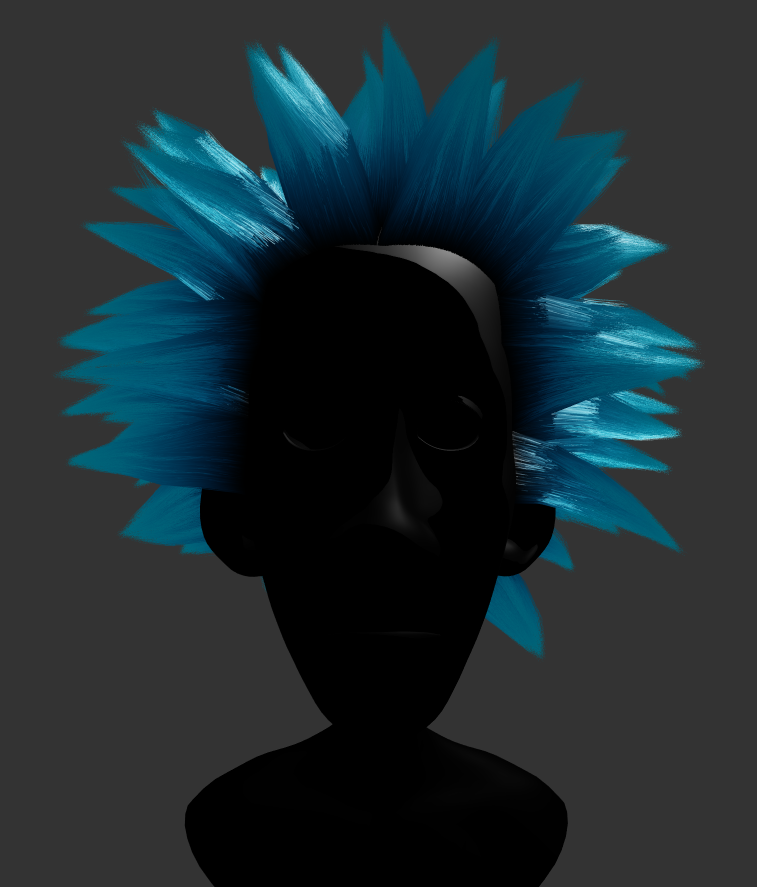
\includegraphics[width=0.45\linewidth]{images/rick}
\hfill
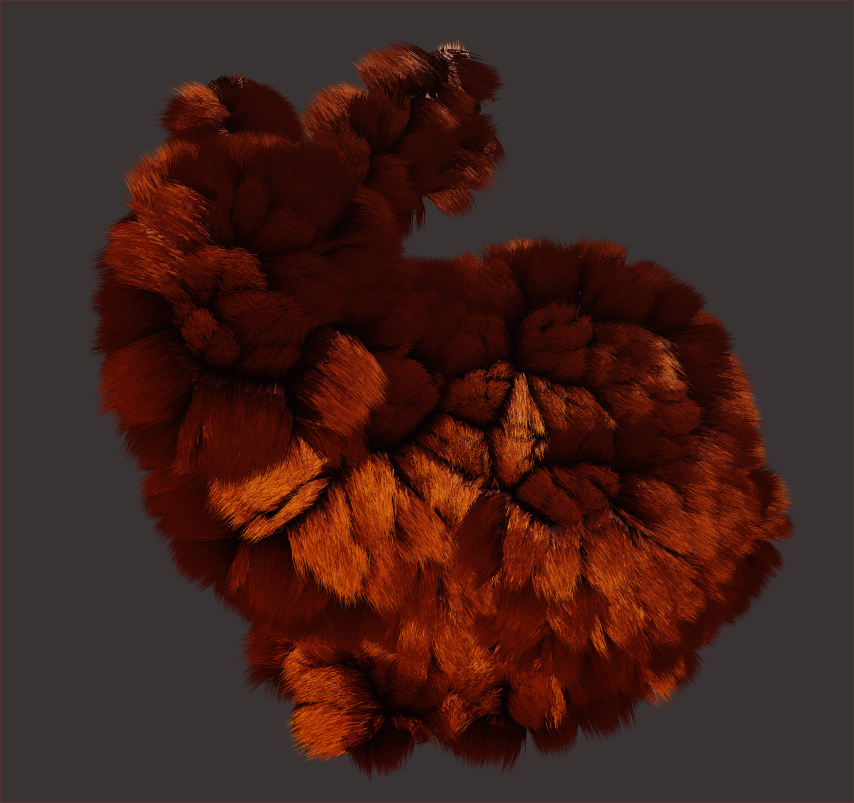
\includegraphics[width=0.45\linewidth]{images/bunny}
\caption{\label{figure:screenshots} Examples of visual output that my system is capable of producing.}
\end{figure}

\begin{figure}[htbp]\centering
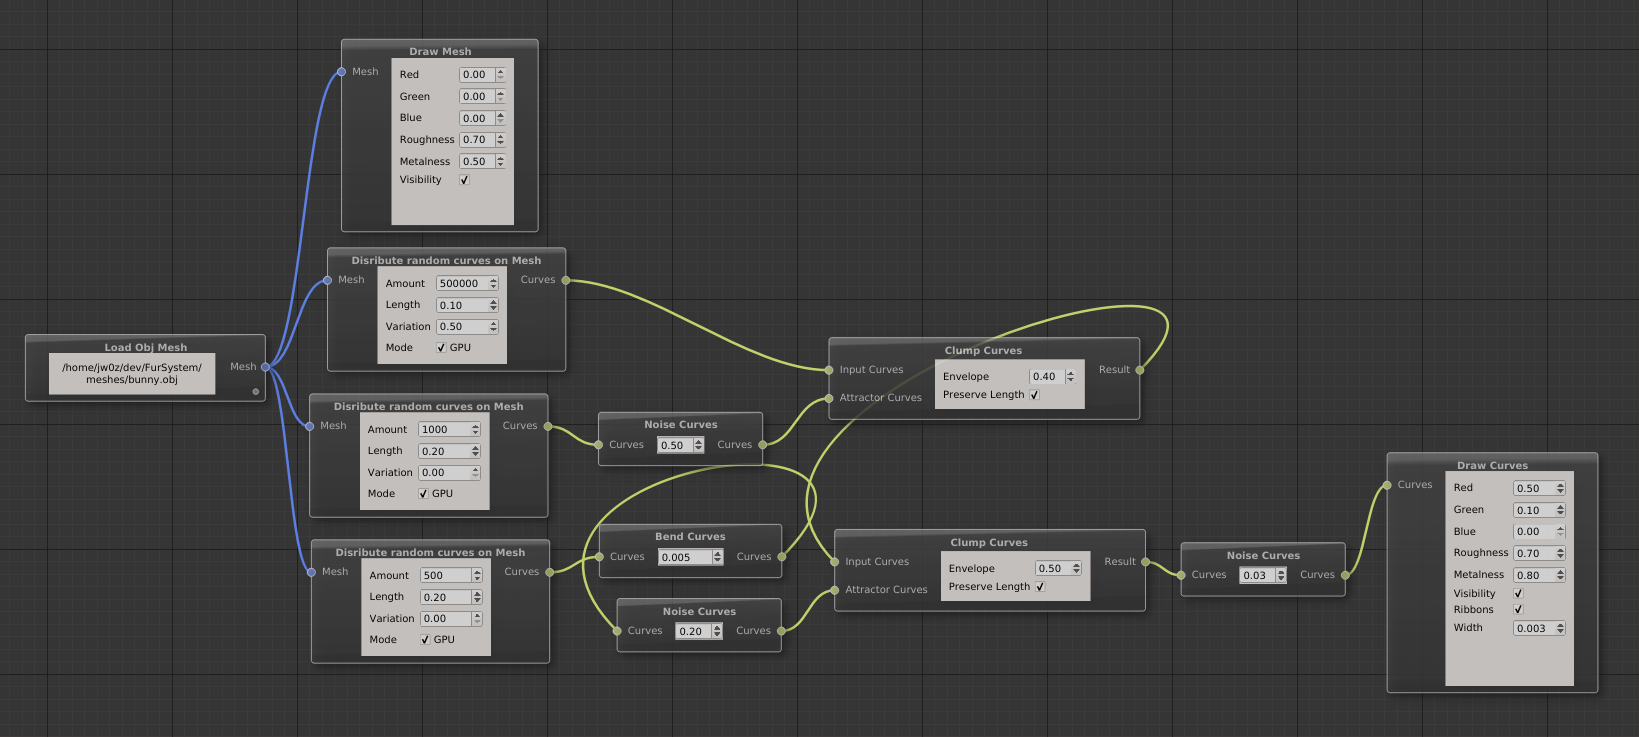
\includegraphics[width=1.0\linewidth]{images/nodes}
\caption{\label{figure:screenshot_gui} The accompanying node graph setup used to create the images in Figure~\ref{figure:screenshots}.}
\end{figure}

\subsection{Performance} \label{sec:performance}

Figures~\ref{figure:distributionPerformance} and~\ref{figure:fullPerformance} show that my system is performant enough to provide real-time feedback, even when dense meshes and high primitive counts are used. Whilst Figure~\ref{figure:distributionPerformance} shows performance gains by utilisizing the GPU over the CPU, note that my CPU implementation is single-threaded, and further performance gains could be made by utilizing multithreading.

It is worth noting that my system is quite inefficient in regards to GPU memory consumption; The node graph setup in Figure~\ref{figure:screenshot_gui} uses 322 MiB of VRAM. This is a result of storing the state of each \texttt{GL\_SHADER\_STORAGE\_BUFFER} in GPU memory, for each of the curve operators used. Whilst this avoids the need for a full graph evaluation each time a parameter is changed, it effectively doubles VRAM usage each time a curve operator is added.

\begin{figure}[htbp]\centering
\begin{center}
\begin{tabular}{||c||c|c|c||}
\hline
Mesh Triangle Count & Primitive Count & CPU Time (ms) & GPU Time (ms)\\
\hline
\hline
16 (Triangle Strip) & 10,000 & 2 - 5 & 1 - 2\\
\hline
 - & 100,000 & 18 - 41 & 8 - 24\\
\hline
 - & 1,000,000 & 120 - 150 & 77 - 110\\
\hline
4968 (Stanford Bunny) & 10,000 & 173 - 211 & 1 - 2\\
\hline
 - & 100,000 & 1718 - 1756 & 12 - 30\\
\hline
 - & 1,000,000 & 17218 - 17259 & 82 - 112\\
\hline
\end{tabular}
\caption{\label{figure:distributionPerformance} Performance metrics showing time taken to distribute varying numbers of primitives, on meshes of varying triangle counts. An Intel Core i7-6700 CPU and an NVIDIA GTX1080 GPU were used for testing.}
\end{center}
\end{figure}

% \begin{figure}[htbp]\centering
% \begin{center}
% \begin{tabular}{||c|c||}
% \hline
% Mesh Triangle Count & GPU Time (ms)\\
% \hline
% \hline
% 16 (Triangle Strip) & 18 - 20\\
% \hline
% 4968 (Stanford Bunny) & 33 - 45\\
% \hline
% 14067 (Utah Teapot) & 76 - 92\\
% \hline
% \end{tabular}
% \caption{\label{figure:fullPerformance} Performance metrics showing the time taken to perform a full graph evaluation on a complex setup, as seen in Figure~\ref{figure:screenshot_gui}, for meshes of varying triangle counts.}
% \end{center}
% \end{figure}

\begin{figure}[htbp]\centering
\begin{center}
\begin{tabular}{||c|c||}
\hline
Mesh Triangle Count & Evaluation Time (ms)\\
\hline
\hline
16 (Triangle Strip) & 69 - 84\\
\hline
4968 (Stanford Bunny) & 81 - 112\\
\hline
14067 (Utah Teapot) & 138 - 228\\
\hline
\end{tabular}
\caption{\label{figure:fullPerformance} Performance metrics showing the time taken to perform a full graph evaluation on a complex setup, as seen in Figure~\ref{figure:screenshot_gui}, for meshes of varying triangle counts. Note that over 500,000 primitives are being processed in this setup.}
\end{center}
\end{figure}

\section{Conclusion} \label{sec:conclusion}

Overall I am pleased with the visual quality and interactivity of my system; currently it provides the basic functionality required to visualise simple hair and fur content, whether it be for a VFX or real-time usage scenario. However, I believe further work is necessary in order to maximise it's performance and usability within a broader production pipeline.

% Currently my system performs all of its computation using OpenGL compute shaders, though better results may be attainable using other APIs such as CUDA or OpenCL.

\subsection{Future Work} \label{sec:futurework}

Unfortunately my system lacks the ability to export curves data, making it virtually unusable within a production pipeline in its current state. A viable file format for this could be \textit{Alembic}~\cite{alembic}, as it natively supports the storage of parametric curves. Integrating alembic support into my system could also allow for animated mesh geometry to be used.

Another desirable addition to my system would be viewport manipulators, similar to the 'Groomable Splines' feature in XGen. This could allow me to implement techniques such as those described in Skippy~\cite{skippy}, which would provide my system with a unique user experience compared to commercially available systems.

Whilst not necessary for usage in a broader pipeline, implementing a physically plausible hair shading model such as those described in \cite{Marschner}, would greatly improve the visual accuracy of my viewport renderings.

\newpage

\bibliographystyle{acmsiggraph}
\bibliography{references}

\newpage
\appendix

\begin{lstlisting}[language=GLSL, label={lst:buffers}, caption={Extract from the Distributor compute shader, showing how the Mesh and Curves buffers are accessed.}]
struct Face
{
	vec4 position[3];
	vec4 normal[3];
	vec4 uv[3];{}
};

layout (std430, binding = 0) buffer facesBuffer
{
	Face faces[];
};

struct Curve
{
	vec4 position[5];
};

layout (std430, binding = 1) buffer curvesBuffer
{
	Curve curves[];
};
\end{lstlisting}

\begin{lstlisting}[language=C++, label={lst:rendercpp}, caption={Extract from the C++ application code showing how Curves are rendered procedurally. \texttt{emptyVAO} is an empty Vertex Array Object, \texttt{curvesSSBO} is a \texttt{GL\_SHADER\_STORAGE\_BUFFER} containing vertex data for multiple curves, and \texttt{indices} is the number of curves in the buffer.}]
glBindVertexArray(emptyVAO);
glBindBufferBase(GL_SHADER_STORAGE_BUFFER, 0, curvesSSBO);
glDrawArrays(GL_POINTS, 0, indices);
\end{lstlisting}

\begin{lstlisting}[language=GLSL, label={lst:renderglsl}, caption={Extract from the curves rendering geometry shader, showing how vertex positions were processed from data stored in a bound \texttt{GL\_SHADER\_STORAGE\_BUFFER}.}]
#version 430 core
layout(points) in;
layout(line_strip, max_vertices = 5) out;

struct Curve
{
	vec4 position[5];
};

layout (std430, binding = 0) buffer curvesBuffer
{
	Curve curves[];
};

uniform mat4 MVP;

void main()
{
	for (int i = 0; i < 5; ++i)
	{
		gl_Position = MVP * vec4(curves[gl_PrimitiveIDIn].position[i].xyz, 1.0);
		EmitVertex();
	}
	EndPrimitive();
}
\end{lstlisting}

\end{document}
